\documentclass{my_paper}
\usepackage{ctex}
\usepackage[textwidth=444bp,vmargin=2.5cm]{geometry}
\usepackage{array}
\usepackage{float}
\usepackage[dvipsnames]{xcolor}
\usepackage{graphicx}
\usepackage{epstopdf}
\usepackage{amsmath}
\usepackage[T1]{fontenc}    
\usepackage{newtxtext, newtxmath}  
\usepackage{caption}
\usepackage[dvipsnames]{xcolor}
\usepackage{listings}
\lstset{
	alsolanguage= matlab,
	alsolanguage= XML,
	tabsize=4, 
	frame=shadowbox, 
	commentstyle=\color{red!50!green!50!blue!50},
	rulesepcolor=\color{red!20!green!20!blue!20},
	keywordstyle=\color{blue!90}\bfseries,
	showstringspaces=false,
	stringstyle=\ttfamily, 
	keepspaces=true, 
	breakindent=22pt, 
	numbers=left,
	stepnumber=1,
	numberstyle={\color[RGB]{0,192,192}\tiny} ,
	numbersep=8pt,  
	basicstyle=\footnotesize, 
	showspaces=false, 
	flexiblecolumns=true, 
	breaklines=true, 
	breakautoindent=true,
	breakindent=4em, 
	escapebegin=\begin{CJK*}{GBK}{hei},escapeend=\end{CJK*},
	aboveskip=1em, 
	tabsize=2,
	showstringspaces=false, 
	backgroundcolor=\color[RGB]{245,245,244},  
	escapeinside=``,  
	fontadjust,
	captionpos=t,	framextopmargin=2pt,framexbottommargin=2pt,abovecaptionskip=-3pt,belowcaptionskip=3pt,
	xleftmargin=4em,xrightmargin=4em, 
	texcl=true,
	extendedchars=false,columns=flexible,mathescape=true
}
\begin{document}
\newpage

\begin{center}
\lunwenbiaoti 

\vspace{2ex}
\zhaiyao
\end{center}

古代玻璃易受埋藏环境的影响而风化,使得化学成分发生变化。现有一批我国古代玻璃文物的相关数据,其已被分为高钾型和铅钡型。本文通过回归分析等方法分析文物风化与其各类特征的关系,并使用聚类分析等统计模型对文物化学成分进行分析,提出了玻璃亚类判别模型。最后结合灰色关联分析与卡方检验,对文物化学成分间联系的差异性进行分析。

针对玻璃化学成分分析的问题,首先将表单中数据进行处理,剔除成分之和不在$85\%-105\%$之间的文物。将采样点对应的玻璃文物分为风化与未风化两组,分别以玻璃类型、纹饰、颜色为依据,绘制三维饼图,进行\textbf{卡方检验},综合二者得出这三种因素与玻璃文物表面风化之间的关系;采用主成分回归分析法对玻璃风化点和未风化点的化学成分进行分析,得到两个主成分,并绘制对应主成分散点图;采用\textbf{多元回归分析法},基于多个主要成分得到回归方程,结合风化点检测数据预测其未风化时的化学成分。

针对已知玻璃重新分类的问题,利用\textbf{支持向量机}分析高钾、铅钡玻璃的分类规律。对于高钾玻璃采用\textbf{R-Q聚类分析方法},建立高钾玻璃类型判别模型,以检测点的二氧化硅($SiO_2$)比例、氧化钾($K_2O$)比例、氧化铜($CuO$)比例为核心,将其分为3个亚类;对于铅钡玻璃使用\textbf{基于二阶聚类分析与K-Means++聚类法的综合聚类方法}建立铅钡玻璃类型判别模型,以检测点的二氧化硅($SiO_2$)比例、氧化铅($PbO$)比例、氧化钡($BaO$)比例为核心,将其分为3个亚类。通过将不同算法的结果进行对比分析,并结合小范围的数据扰动,得到5\%波动范围内稳定的匹配率,其高达83.6\%,证明了分类模型的合理性与稳定性。

针对鉴别未知玻璃类别的问题,首先将附件中表单三的数据代入支持向量机,得出A2、A3、A4、A5、A8属于铅钡玻璃;A1、A6、A7属于高钾玻璃的初步分类。然后分别对两种玻璃数据使用\textbf{逐步判别分析法},得出六种亚类各自的判别函数,并初步判断得A6、A7属于亚类1,A1属于亚类2,A2、A3、A4属于亚类4,A5属于亚类5,A8属于亚类6,即将八个未知类别的玻璃文物归入\textbf{两个大类中的五个亚类}。同时采用R-Q型聚类分析法进行结果对比分析,并结合小范围的数据扰动,得到5\%波动范围内稳定的匹配率,其接近100\%,证明了鉴别模型的合理性与稳定性。

针对不同类别的玻璃成分关联性分析问题,首先采用\textbf{灰色关联分析方法},计算其余化学成分与二氧化硅($SiO_2$)含量的灰色关联系数,进而求出对应的\textbf{灰色加权关联度}。然后,随机将两个不同亚类分为一组,逐组对其求得的关联度进行卡方检验,最终发现高钾玻璃与铅钡玻璃的亚类间的化学成分关联关系差异较大。

本文使用了多种统计模型,使建立的分类模型、鉴别模型等稳定性和鲁棒性更好。同时对模型的优缺点进行评价,综合考虑各模型的拟合能力和应用前景,分析出所构建的模型在考古挖掘、矿石分析等领域具有潜在的应用价值。



\begin{guanjianci}
 \quad \textbf{支持向量机}\quad \textbf{逐步判别分析}\quad \textbf{回归分析}\quad \textbf{综合聚类分析}\quad \textbf{灰色关联分析}
\end{guanjianci}

%----------- 正文 ----------
%----------- 一、问题重述 ----------
\newpage
\section{一、问题重述}
我国古代玻璃吸收了外来的制作工艺,在本土取材制作,其外表与外来的玻璃制品类似,但化学成分却不相同。 由于玻璃的主要原料石英砂(主要成分为二氧化硅)的熔点较高,在炼制时需要添加助熔剂以使其熔化温度降低。我国发明的铅钡玻璃使用铅矿石作为助熔剂,含有较多氧化铅($PbO$)、氧化钡($BaO$);而钾玻璃则采用碳酸钾等含钾量高的物质。

埋藏环境的影响使得古代玻璃容易风化。风化过程是内部与外部大量元素交换的过程,玻璃的成分比例在此过程中产生变化,影响对其类别的判断。

现有一批我国古代玻璃制品的相关数据,已知其分为高钾玻璃和铅钡玻璃两种类型,根据附件中相关数据,解决下列问题:

\textbf{问题1} 根据表格数据,分析玻璃的类型、玻璃的纹饰、玻璃的颜色与文物表面风化情况的关系;基于玻璃类型,分析文物化学成分含量与有无风化的关系,并得出统计规律;以风化点的检测数据为依据,预测风化前的化学成分含量.

\textbf{问题2} 根据附件数据分析两种玻璃的分类规律原理;并对每个类别依据合适的化学成分划分出一定数目的亚类,同时需要给出具体的划分方法和结果,并分析分类结果的合理性,分类的灵敏度。

\textbf{问题3} 根据已经建立的模型,基于附件表单3中未知类别的玻璃文物的化学成分,鉴别其所属类型,并分析分类结果的合理性,分类方法的敏感度。
                            
\textbf{问题4} 分析不同亚类的玻璃文物样品化学成分之间的关联关系,并比较不同亚类之间的化学成分关联关系的差异性.

%----------- 二、问题分析 ----------
\section{二、问题分析}
\subsection{数据预处理}
基于题目有效数据的定义,将附件表单二中所有采样点的化学成分比例进行累加,筛选出成分比例之和为79.41\%的采样点15以及成分比例之和为71.89\%的采样点17,进而将其从表单中剔除。
\subsection{问题一的分析}
对于问题一,首先可定性地把采样点对应的玻璃文物分为风化与未风化两组,分别以玻璃类型、纹饰、颜色为依据,使用MATLAB绘制三维饼图;定量地通过卡方检验,得出三种因素与表面风化的显著性影响,综合二者得出这三种因素与文物表面风化之间的关系。

之后基于文献\cite{崔剑锋2009湖南沅水流域战国时期楚墓出土古代玻璃器的成分分析},可采用主成分回归分析法对风化玻璃和未风化玻璃的化学成分进行分析,求解出一定量主成分,并可绘制主成分散点图进行直观判断。

为预测未风化前样本点的化学成分,通过多元回归分析模型,建立玻璃文物的化学组分内部线性关系,运用内部线性关系反推得到部分较为显著的化学组分。

\subsection{问题二的分析}
问题二首先要求对高钾玻璃、铅钡玻璃的划分规律进行分析。采用支持向量机的方法,选取31号、08号严重风化点、26号严重风化点、54号严重风化点、16号、12号采样点作为待测点,将待测点与剩余的61个采样点的数据进行标准化处理,计算已分类的数据的均值向量与标准差向量,得出线性分类函数,即为高钾玻璃、铅钡玻璃的划分规律。

对于高钾玻璃,使用R-Q聚类分析方法,首先对玻璃文物的14项指标,运用MATLAB计算相关系数矩阵,并对其进行R型聚类,将14项指标分为9个类别,再根据这9类指标对18个采样点进行Q型聚类分析,根据聚类树形图将这18个采样点分为三类。

对于铅钡玻璃,采用基于二阶聚类分析与K-Means聚类法的亚类划分方法,首先检验数据的分布特性与独立性,其次调用SPSS软件进行二阶聚类分析得到推荐分类数与轮廓测量值,然后基于推荐分类数分别进行K-Means聚类分析与QR聚类分析,最后比照二者结果,对亚类划分做出一定的修正,得出结论。

\subsection{问题三的分析}
问题三可先采用SVM支持向量机的方法确定未知玻璃文物属于高钾类别还是铅钡类别,再基于两种类别分别建立基于逐步判别分析方法的文物类型鉴别模型,将未知玻璃文物代入模型,得到初步判定结果。再结合多种聚类方法进行检验,得出最终玻璃文物所属类别的判定结果。

采用逐步判别法选择分析变量。经过多步判别分析,分别选取高钾玻璃变量,铅钡玻璃的变量进入判别方程,建立文物鉴别模型。
\subsection{问题四的分析}
问题四首先采用灰色关联分析方法,计算其余化学成分与二氧化硅($SiO_2$)含量的灰色关联度,并求出灰色加权关联度。其次,将求得的关联度以两个类别为一组进行卡方检验,得出高钾型玻璃与铅钡型玻璃的亚类间的化学成分关联关系差异较大的结论。

%----------- 三、模型假设 ----------
\section{三、模型假设}
\noindent
$\bullet$ 假设无风化的文物表面没有风化部位\\
$\bullet$ 假设回归分析的变量服从独立的正态分布\\ 
$\bullet$ 认为未检测到的成分在样本中不存在\\
$\bullet$ 假设同文物不同取样点的数据均符合类型划分
%----------- 四、符号说明 ----------
\section{四、符号说明}

\begin{table}[H]
    \centering
    \begin{tabular}{p{2.0cm}<{\centering}p{9.0cm}<{\centering}p{2.0cm}<{\centering}}
    \hline
    符号 & 说明  \\ %换行 
    \hline
    F1&     第一主成分含量  \\
    F2&     第二主成分含量   \\
    $\mu$&   样本点的均值向量 \\
    $\sigma$& 样本点的标准差向量 \\
    $x_I$  &采样点对应成分的比例\\
    $r_i$ &灰色加权关联度 \\
    $f_i$ & 各亚类判别函数 \\\hline
    \end{tabular}
\end{table}

%----------- 五、模型的建立与求解 ----------
\section{五、模型的建立与求解}


\subsection{问题一模型的建立与求解}
\subsubsection{基于统计图表的玻璃风化因素分析}
从定性角度,对于附录1中的文物,将其分为高钾玻璃和铅钡玻璃两组来分别统计纹饰、颜色和风化与否的关联。使用MATLAB绘制饼图,以直观反映各种因素的影响程度。绘制出的图如下:
\begin{figure}[H]
\centering 
\includegraphics[width=0.49\textwidth]{饼图1.jpg} 
\includegraphics[width=0.49\textwidth]{饼图2.jpg} 
\caption{玻璃种类、颜色、纹饰与风化的比例关系} 
\end{figure}

通过对图1的八个子图进行分析,可知:

就纹饰而言:风化和未风化的铅钡玻璃纹饰的比例相差较小,前者A类纹饰与C类纹饰的比例分别为37.5\%与62.5\%,后者A类纹饰与C类纹饰的比例分别为41.7\%与58.3\%,差值在5\%以内;而风化和未风化的高钾玻璃纹饰的比例相差较大,前者均为B类纹饰,后者A类纹饰与C类纹饰的比例为60\%与40\%。\par
就颜色而言:风化与否的玻璃颜色差异均较明显。对于风化的铅钡玻璃,浅蓝色比例最多,达到50\%,浅绿色比例最小,不存在绿色和深蓝色,其余颜色比例相近,而对于未风化的铅钡玻璃,浅蓝色的比例最多,达到33\%,同时深绿色、浅绿色、紫色占比次之,而深蓝色和绿色占比均最小,不存在蓝绿色和黑色;对于风化的高钾玻璃,其颜色均为蓝绿色,而对于未风化的高钾玻璃,蓝绿色占比最多,达到60\%,其次是浅蓝色,占比20\%,之后是深蓝和深绿色,均占比10\%,其余四种颜色不存在。\par
从定量角度,由于玻璃类型、纹饰、颜色、表面风化均为定类变量,所以为分析其与表面风化之间的关系,可以采用卡方检验的方式来分析其关系。\par
卡方检验的结果如表\ref{卡方检验结果}所示:
\begin{table}[H]
    \centering
    \caption{玻璃文物的类型、纹饰、颜色与表面风化的卡方检验结果}
    \label{卡方检验结果}
    \begin{tabular}{llll}
    \hline
        & $X^2$ & 经校正$X^2$ & 显著性P \\ \hline
        玻璃类型 & 3.861 & 2.758 & 0.049 \\ 
        纹饰种类 & 5.72 & 5.72 & 0.057 \\ 
        玻璃颜色 & 7.011 & 7.011 & 0.428 \\ \hline
    \end{tabular}
\end{table}

由表可知,对于玻璃的类型与玻璃的颜色,其对于表面风化的显著性概率P均小于0.05,故认为玻璃的类型与玻璃的颜色与文物表面是否风化有显著性关系;对于纹饰的类型,其对于表面风化的显著性概率P大于0.05,故认为纹饰的类型与文物表面是否风化无显著性关系。
结合定性与定量的分析,可以得出三点结论:
\begin{enumerate}
    \item 玻璃的种类不同,对文物表面是否风化有显著性影响。
    \item 同种玻璃的纹饰不同,对文物表面是否风化无较为显著的影响。就铅钡玻璃而言,B类纹饰的玻璃风化的概率极小,而A、C两类纹饰的玻璃均可能风化,且后者风化的概率更大;就高钾玻璃而言,B类纹饰的玻璃风化的概率较大,A、C两类纹饰的玻璃风化概率较小,故纹饰类型对文物表面风化的影响较小。
    \item 玻璃的颜色不同,对文物表面是否风化有显著性影响。就铅钡玻璃而言,绿色和深蓝色风化的概率极小,浅蓝色的概率较大;就高钾玻璃而言,蓝绿色风化的概率极大,其余颜色风化的概率较小。
\end{enumerate}
\subsubsection{基于主成分回归分析法的玻璃化学成分统计规律分析}
由题意知分析样品表面化学成分含量的统计规律时,需考虑样品的风化与否。通过查阅文献\cite{崔剑锋2009湖南沅水流域战国时期楚墓出土古代玻璃器的成分分析}和\cite{温睿新疆巴里坤石人子沟遗址群出土玻璃珠的成分分析}知,可采用主成分回归分析法进行分析,其处理思路如图\ref{分析思路}示:
\begin{figure}[H]
    \centering
    \includegraphics[width=0.85\textwidth]{基于主成分分析的成分含量规律分析思路.jpg}
    \caption{主成分回归分析化学成分统计规律的思路}
    \label{分析思路}
\end{figure}
\textbf{对未风化玻璃化学成分主成分回归分析的模型建立及求解过程如下:}\par
\textbf{Step 1} \par
数据处理:设表单二有效数据中未风化玻璃各个化学成分构成的矩阵为A,对矩阵A进行数据标准化处理,然后进一步求解得到对应的相关系数矩阵R,xi表征附件表单二第i个成分含量,求解得相关系数表如表\ref{未风化玻璃化学成分相关系数表}所示:

\begin{table}[H]
    \centering
    \caption{未风化玻璃化学成分相关系数表}
    \label{未风化玻璃化学成分相关系数表}
    \begin{tabular}{lllllllll}
    \hline
         &x1 & x2 & x3 & x4 & x5 & x6 & x9 & x10 \\ \hline
        x1 & 1.000  & -0.423  & -0.094  & 0.106  & 0.089  & 0.255  & -0.860  & -0.554  \\ 
        x2 & -0.423  & 1.000  & -0.794  & -0.875  & -0.916  & -0.952  & 0.822  & 0.764  \\
        x3 & -0.094  & -0.794  & 1.000  & 0.980  & 0.971  & 0.932  & -0.357  & -0.711  \\ 
        x4 & 0.106  & -0.875  & 0.980  & 1.000  & 0.986  & 0.981  & -0.527  & -0.823  \\ 
        x5 & 0.089  & -0.916  & 0.971  & 0.986  & 1.000  & 0.985  & -0.550  & -0.751  \\ 
        x6 & 0.255  & -0.952  & 0.932  & 0.981  & 0.985  & 1.000  & -0.671  & -0.840  \\ 
        x9 & -0.860  & 0.822  & -0.357  & -0.527  & -0.550  & -0.671  & 1.000  & 0.730  \\ 
        x10 & -0.554  & 0.764  & -0.711  & -0.823  & -0.751  & -0.840  & 0.730  & 1.000 \\  \hline
    \end{tabular}
\end{table}

进而求解R的特征值与特征向量,得到表格\ref{未风化玻璃相关系数矩阵特征}如下:
\begin{table}[H]
    \centering
    \caption{未风化玻璃相关系数矩阵特征}
    \label{未风化玻璃相关系数矩阵特征}
    \begin{tabular}{lllllll}
    \hline
        成分 & 特征值 & 特征值百分比 & 累积 \% & 方差 & 方差百分比 \% & 累积 \% \\ \hline
        1 & 7.91 & 79.104 & 79.104 & 5.672 &  56.725 & 56.725 \\ 
        2 & 1.55 & 15.508 & 94.612 & 4.025 &  40.246 & 96.971 \\ \hline
    \end{tabular}
\end{table}
由表可知,前两个主成分的累计贡献率已达到94.612\%,已能较好解释原有变量,故仅选取两个主成分,即氧化钾含量和氧化铅含量,分别设为F1和F2,则得到

$
    F1=0.380*V2 + 0.961*V3 + 0.881*V4 + 0.956*V5 + 0.953*V6 + 0.991*V7 - 0.754*V10 - 0.890*V11
$

$
    F2=-0.922*V2+0.082*v3+0.469*V4+0.284*v5+0.290*V6+0.129*v7+0.635*V10+0.204*V11
$

\textbf{Step 2} 散点图绘制:\par
根据已得到的F1和F2公式,代入所有未风化的点对应数据,得到所有未风化的点对应的F1和F2,并据此绘制散点图与95\%置信椭圆,如图\ref{未风化}所示:
\begin{figure}[H]
\centering
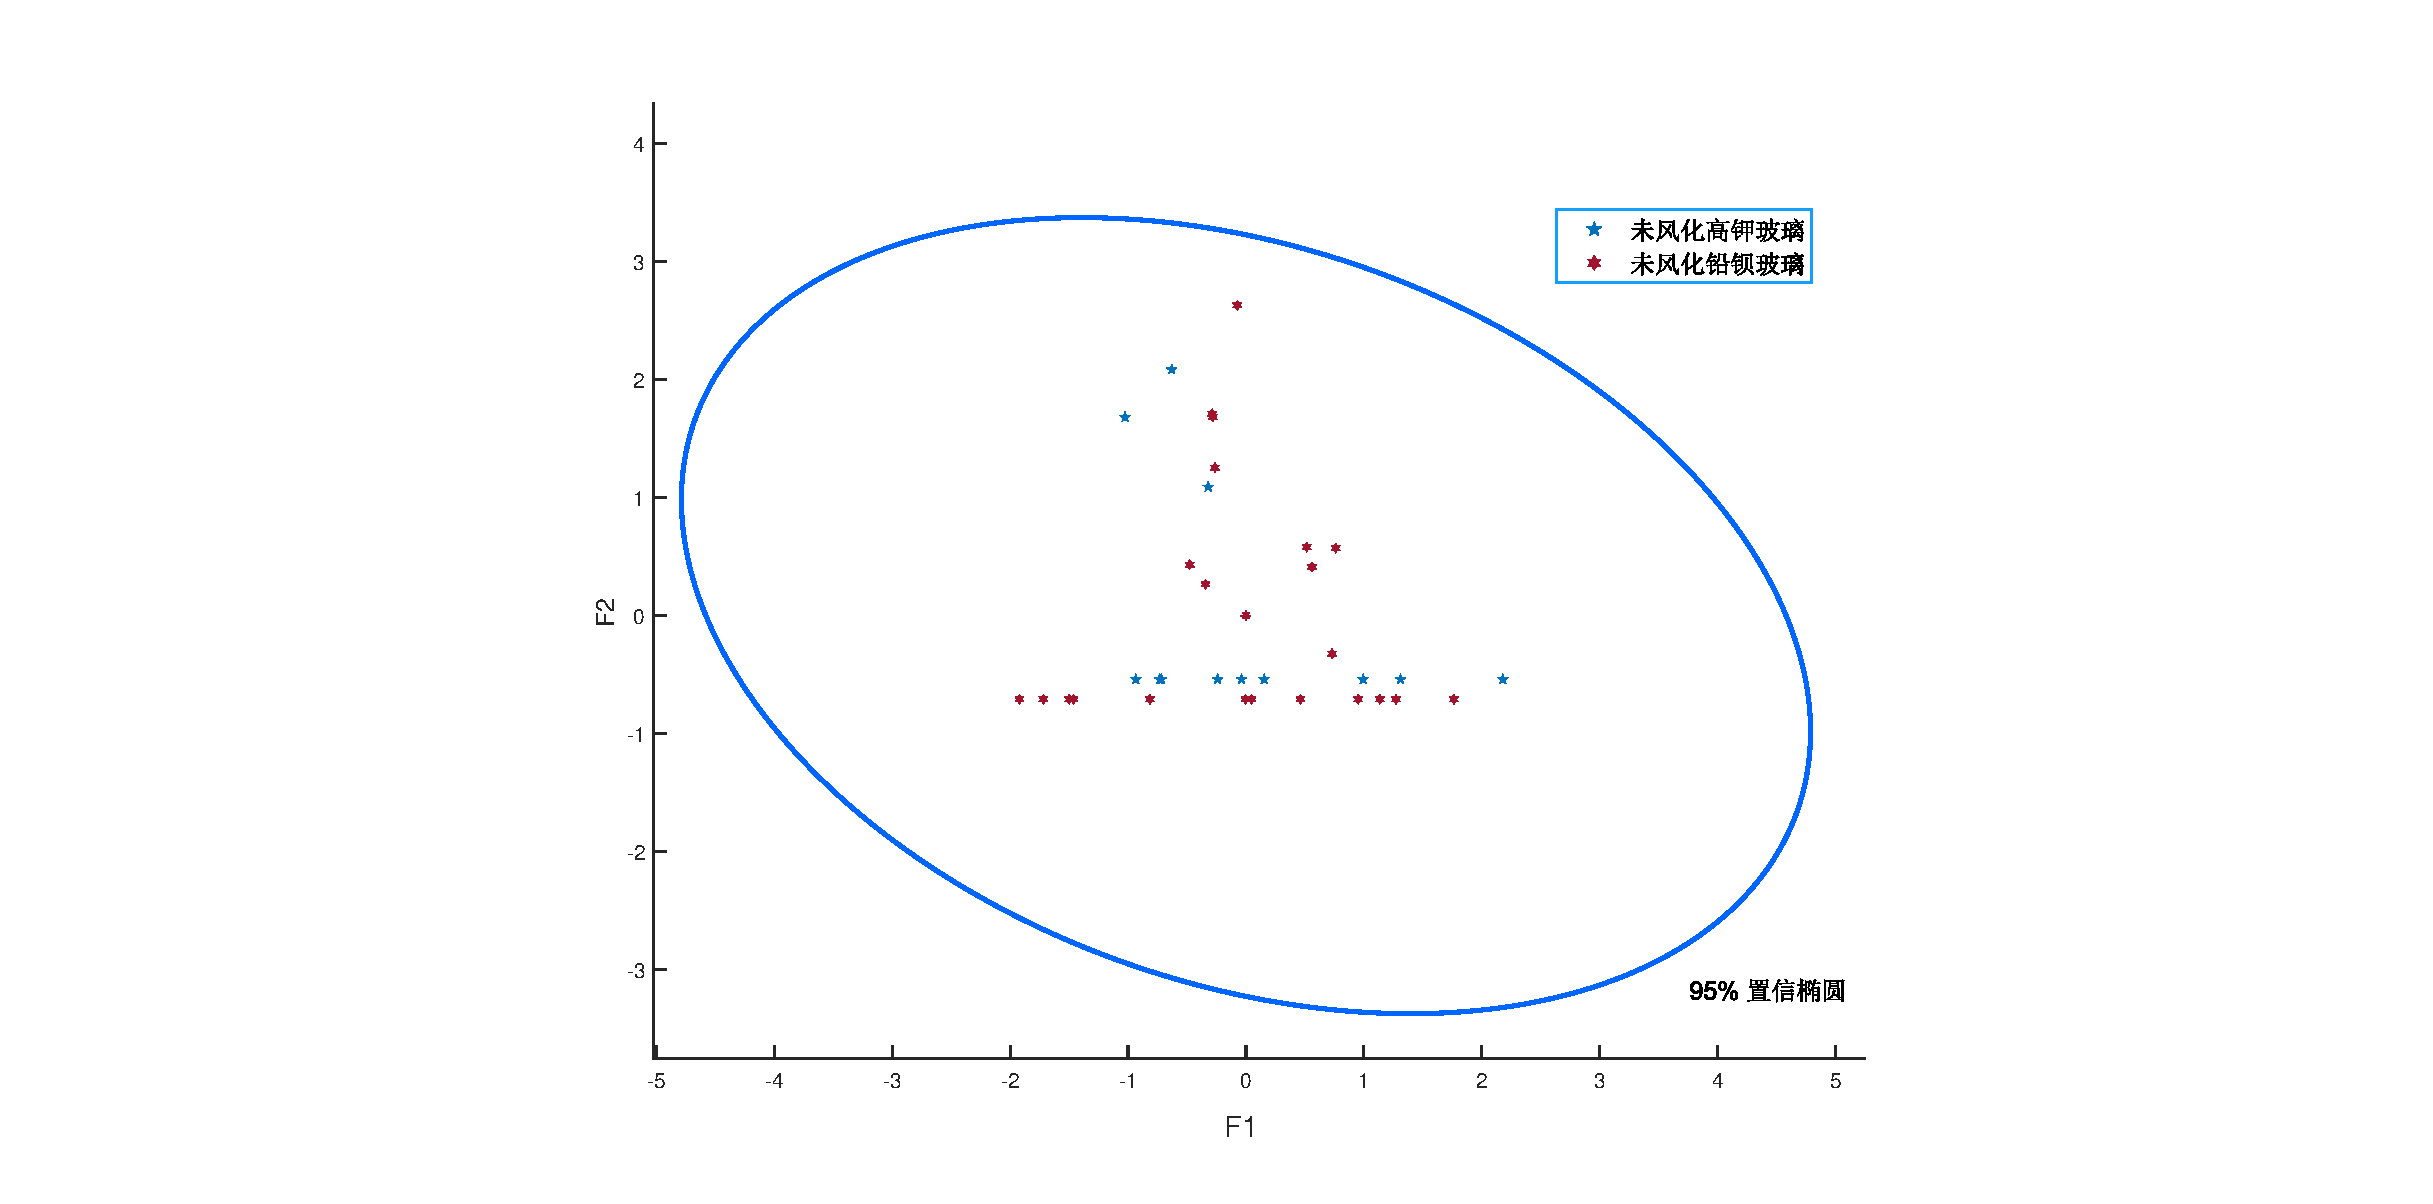
\includegraphics[width=0.9\textwidth]{未风化.eps}
\caption{未风化玻璃化学组成第一、第二主成分散点图}
\label{未风化}
\end{figure}
由图\ref{未风化}可知,所有点均位于95\%置信椭圆内,说明算法选择得当。同时高钾玻璃的F1较集中,F2较分散,即其氧化钾($K_2O$)含量较高,氧化铅(PbO)含量较低;铅钡玻璃的F1较分散,F2较集中,即其氧化钾($K_2O$)含量较高,氧化铅(PbO)含量较低,符合实际情况。\par

\textbf{同理,对于已风化玻璃的化学成分,可以采取相同方法建立模型及求解,过程如下:}\par

\textbf{Step 1} \par
数据处理:设表单二有效数据中风化玻璃各个化学成分构成的矩阵为B,对矩阵B进行数据标准化处理,然后进一步求解得到对应的相关系数矩阵R1,xi表征附件表单二第i个成分含量,进而求解得R1相关系数表如下表\ref{风化玻璃化学成分相关系数表}所示:
\begin{table}[H]
 \centering
 \caption{风化玻璃化学成分相关系数表}
  \label{风化玻璃化学成分相关系数表}
 \begin{tabular}{llllllllllll}
 \hline
            & X1 & X2 & X3 & X4 & X5 & X6 & X7 & X8 & X9 & X10 \\ \hline
         X1 & 1.000  & -0.997  & -0.713  & 0.718  & -0.176  & 0.995  & 0.558  & -0.925  & -0.611  & -0.998  \\ 
         X2 & -0.977  & 1.000  & -0.661  & -0.667  & 0.105  & -0.985  & -0.497  & 0.896  & 0.553  & 0.992  \\ 
         X3 & 0.713  & -0.661  & 1.000  & 0.987  & -0.815  & 0.781  & 0.980  & -0.926  & -0.991  & -0.673  \\ 
         X4 & 0.718  & -0.667  & 0.987  & 1.000  & -0.811  & 0.786  & 0.978  & -0.928  & -0.990  & -0.679  \\ 
         X5 & -0.176  & -0.105  & -0.815  & -0.811  & 1.000  & -0.276  & -0.915  & 0.536  & 0.887  & 0.121  \\ 
         X6 & 0.995  & -0.985  & 0.781  & 0.786  & -0.276  & 1.000  & 0.640  & -0.959  & -0.689  & -0.988  \\ 
         X7 & 0.558  & -0.497  & 0.980  & 0.978  & -0.915  & 0.640  & 1.000  & -0.831  & -0.998  & -0.511  \\ 
         X8 & -0.925  & 0.896  & 0.926  & -0.928  & 0.536  & -0.959  & -0.831  & 1.000  & 0.866  & 0.903  \\ 
         X9 & -0.611  & 0.553  & 0.991  & -0.990  & 0.887  & -0.689  & -0.998  & 0.866  & 1.000  & 0.567  \\ 
         X10 & -0.998  & 0.992  & 0.673  & -0.679  & 0.121  & -0.988  & -0.511  & 0.903  & 0.567  & 1.000 \\ \hline
    \end{tabular}
\end{table}

\newpage
进而求解R1的特征值与特征向量,得到表格\ref{风化玻璃化学成分相关系数表特征}如下:
\begin{table}[H]
    \centering
    \caption{风化玻璃化学成分相关系数表特征}
    \label{风化玻璃化学成分相关系数表特征}
    \begin{tabular}{lllllll}
    \hline
       成分 & 特征值 & 特征值百分比 & 累积 \% & 方差 & 方差百分比 \% & 累积 \% \\ \hline
        1 & 6.007 & 75.093 & 75.093 & 6.007 & 75.093 & 75.093 \\ 
        2 & 1.703 & 21.289 & 96.382 & 1.703 & 21.289 & 96.382 \\ 
        3 & 0.189 & 2.702 & 99.084 & 0.189 & 2.702 & 99.084 \\ \hline
    \end{tabular}
\end{table}

由表可知,前两个主成分的累计贡献率已达到96.382\%,方差百分比已经达到94.848\%,能充分反映数据特征,故仅选取两个主成分,即氧化钾含量和氧化铅含量,同理可以分别用F1和F2替代,则得到

$
    F1=0.878*V2-0.842*V3+0.962*V4+0.964*V5-0.625*V6+0.922*V7+0.887*V9-0.994*V10-0.915*V11-0.850*V13$
    
$
    F2=-0.479*V2+0.540*V3+0.274*V4+0.267*V5-0.780*V6-0.386*V7+0.462*V9+0.110*V10-0.403*V11+0.526*V13
$

\textbf{Step 2} 散点图绘制:\par
根据已得到的F1和F2公式,代入所有已风化的点对应数据,得到所有已风化的点对应的F1和F2,并据此绘制散点图与95\%置信椭圆,如图\ref{已风化}所示:
\begin{figure}[H]
\centering
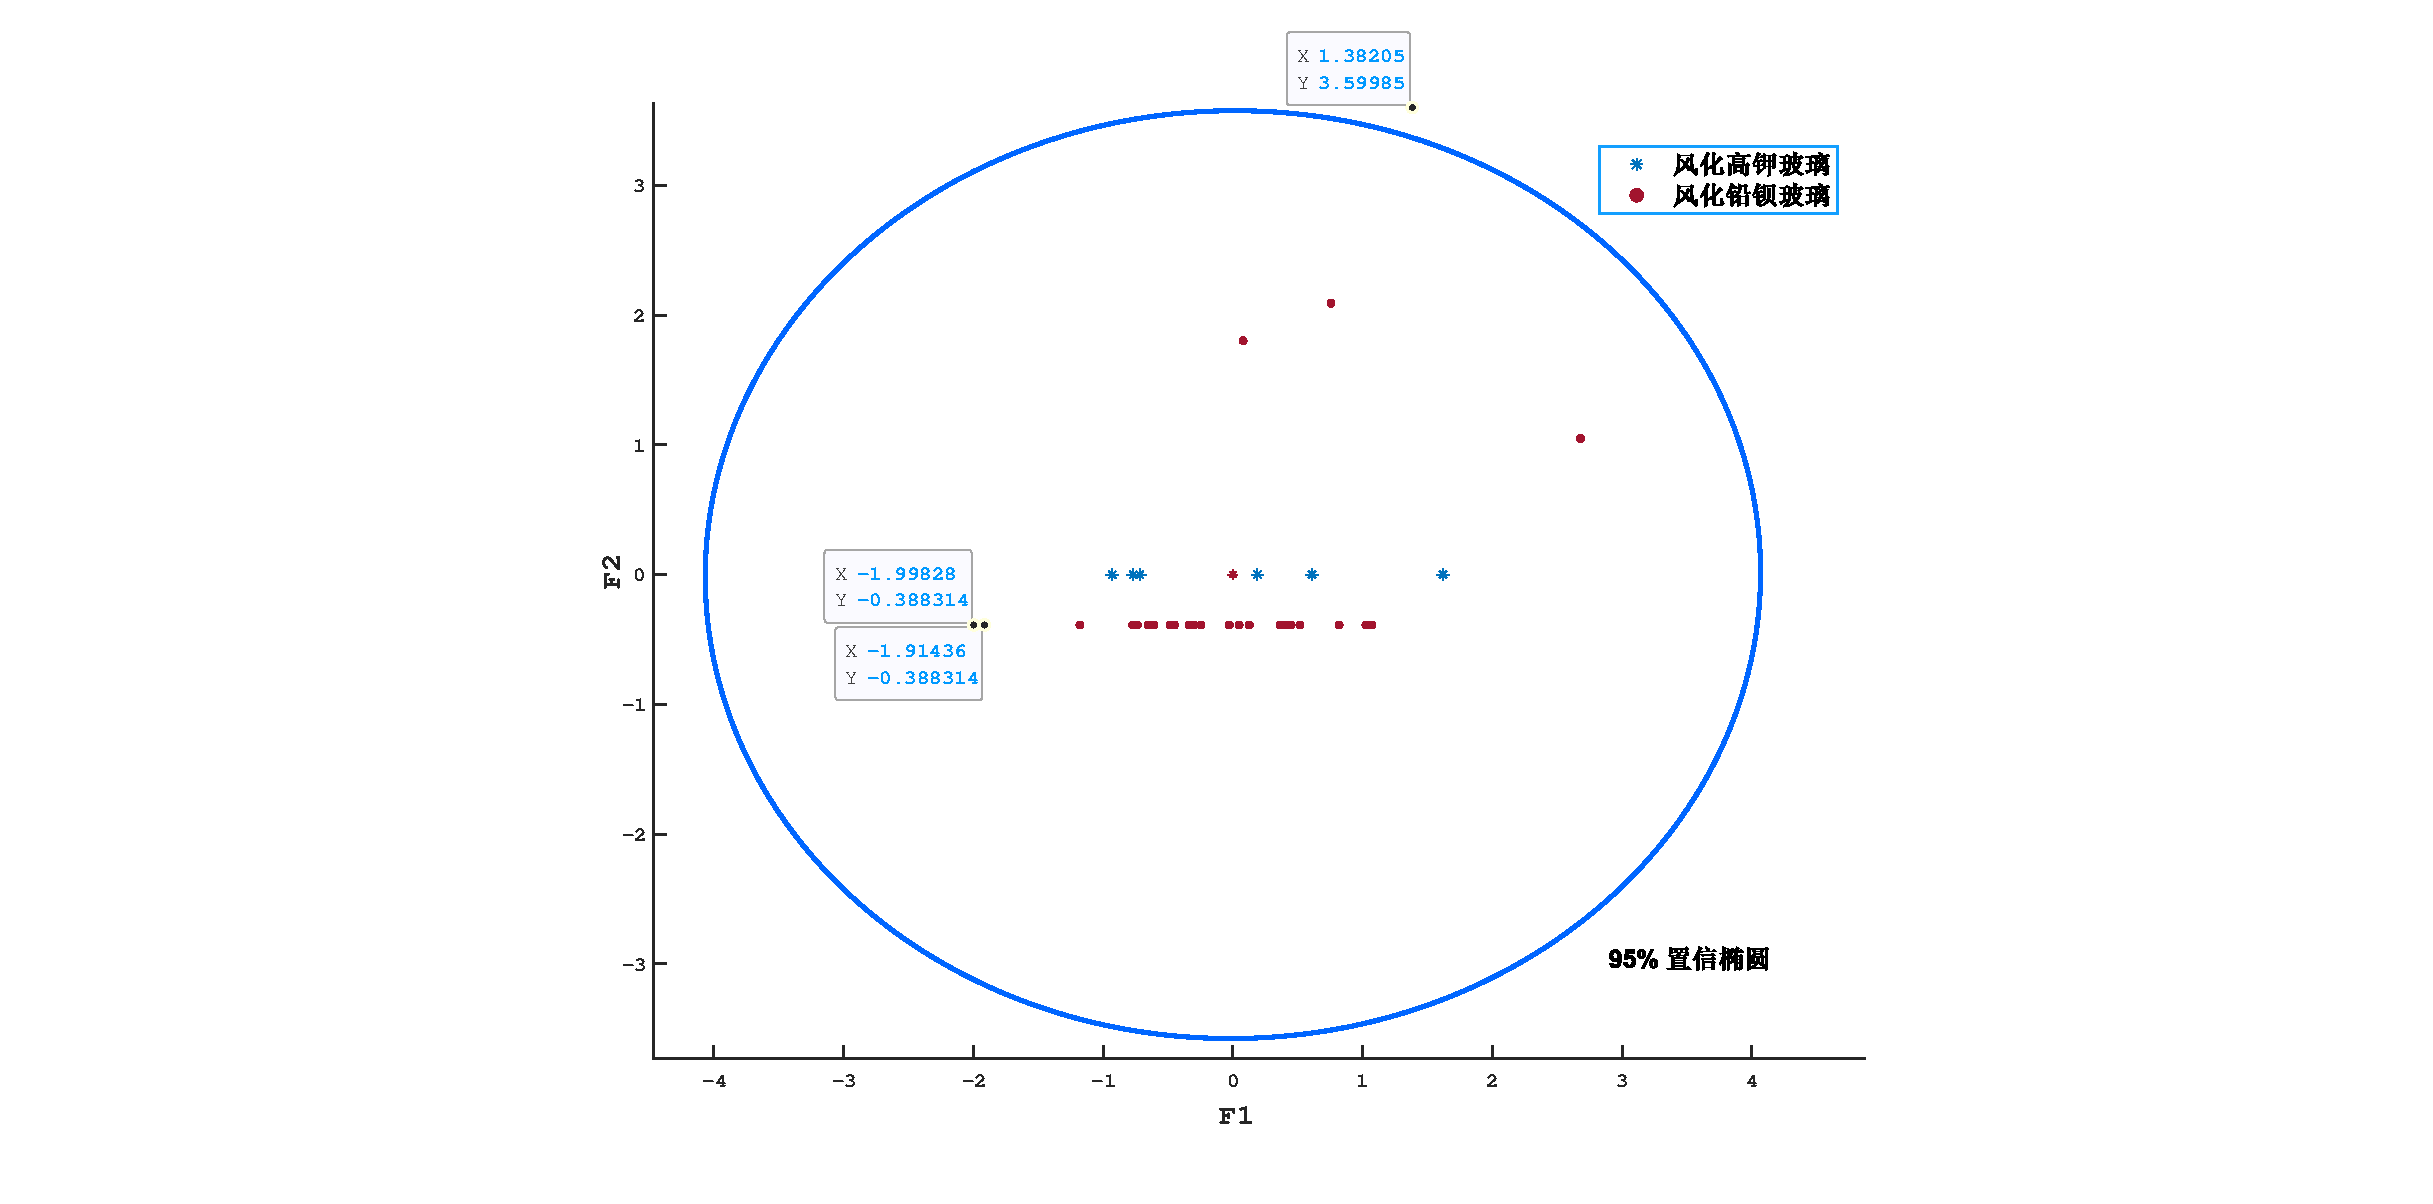
\includegraphics[width=0.9\textwidth]{已风化.eps}
\caption{已风化玻璃化学组成第一、第二主成分散点图}
\label{已风化}
\end{figure}
由图\ref{已风化}可知,几乎所有点均位于95\%置信椭圆内,说明算法选择得当。同时高钾玻璃的F1、F2均较集中,即其氧化钾($K_2O$)含量较高,氧化铅含量($PbO$)稳定;铅钡玻璃的F1较分散,F2较集中,即其氧化钾($K_2O$)含量较高,氧化铅($PbO$)含量较低,符合实际情况。\par
同时针对偏离中心最远的三个点,最左侧的两个采样点编号点分别为8与26,且据附件表单二知其均为严重风化点,同时置信椭圆外的采样点36为风化点,所以可以推测采样点36为严重风化点。
\subsubsection{基于多元回归分析的风化文物成分预测模型}
分析表单2,所有的玻璃采样点均探测出二氧化硅成分,故选用二氧化硅作为多元回归分析模型的因变量$y$。

多元线性回归分析\cite{司守奎2011数学建模算法与应用}的模型为:

$$\left\{\begin{array}{l}
y=\beta_{0}+\beta_{1} l_{1}+\cdots+\beta_{m} l_{m}+\varepsilon \\
\varepsilon \sim N\left(0, \sigma^{2}\right)
\end{array}\right.$$

模型中的参数 $ \beta_{0}, \beta_{1}, \cdots, \beta_{13} $ 仍用最小二乘法估计, 即应选取估计值  $\beta_{j} $, 使 当 $\beta_{j}=\hat{\beta}_{j}, \quad j=0,1,2, \cdots, 13 $ 时, 误差平方和

$$Q=\sum_{i=1}^{n} \varepsilon_{i}^{2}=\sum_{i=1}^{n}\left(y_{i}-\beta_{0}-\beta_{1} l_{i 1}-\cdots-\beta_{13} l_{i 13}\right)^{2}$$ \\
最小,利用SPSS解得回归方程为:

$$ y= 95.871-4.121 x_4-0.659x_6-0.925x_9-1.496x_{10}$$

根据风化样本点的化学成分,运用内部线性关系反推得到部分较为显著的化学组分,结果如表\ref{预测}

\begin{table}[H]
    \centering
    \begin{tabular}{llllll}
    \hline
        采样点 & 二氧化硅($SiO_2$) & 氧化钙($CaO$) & 氧化铝($Al_2O_3$) & 氧化铅($PbO$) & 氧化钡($BaO$) \\ \hline
        8 & 74.39891 & 3.19 & 3.47 & 2.13 & 2.72 \\ 
        26 & 75.40489 & 3.01 & 3.18 & 2.52 & 2.43 \\ 
        54 & 61.41192 & 4.54 & 3.65 & 5.79 & 5.34 \\ \hline
    \end{tabular}
    \caption{预测结果}
    \label{预测}
\end{table}

\subsection{问题二模型的建立与求解}
\subsubsection{基于支持向量机的玻璃分类规律分析}
对剔除15号与17号文物的表单2进行数据处理。在各种类型的文物中各选取一个样本作为待测样本,分别为31号、08号严重风化点、26号严重风化点、54号严重风化点、16号、12号采样点。对于剩余数据使用支持向量机进行分析,其思路如图\ref{向量机}所示:
\begin{figure}[H]
    \centering
    \includegraphics[width=0.9\textwidth]{支持向量机思路.jpg}
    \caption{支持向量机划分玻璃种类思路}
    \label{向量机}
\end{figure}

用$i=1,2,\dots,61 $分别表示61个文物采样点,第$i$个采样点的第$j$个指标的取值为$a_{ij}$。$y_i=1$表示第1类,$y_i=-1$表示第2类.

计算得已知61个样本点的均值向量

$=\boldsymbol{\mu}=[\mu_1,\mu_2,\dots,\mu_{14}]$

$=[49.7323,0.8289,1.7672,2.5061,0.7089,4.1646,0.8461,1.9616,24.6157,7.5287,2.4648,0.2449,0.0854,0.1544]$

61个样本点的标准差向量

$\boldsymbol{\sigma}=[\sigma_1,\sigma_2,\dots,\sigma_{14}]$

$=[22.8604,1.7103,3.6950,2.2823,0.6612,3.1383,1.1184,2.3243,19.4185,7.2862,3.2792,0.2464,0.3528,0.6184]$

对所有样本点数据利用如下公式进行标准化处理:
$$ \tilde{a}_{i j}=\frac{a_{i j}-\mu_{j}}{\sigma_{j}}, i=1,2, \cdots, 61 ; j=1,2, \cdots, 14.$$

对应地,称
$$\tilde{x_{j}}=\frac{x_{j}-\mu_{j}}{s_{j}}, j=1,2, \cdots, 14 $$

为标准化指标变量。记$\tilde{x}=\left[\tilde{x}_{1}, \tilde{x}_{2}, \cdots, \tilde{x}_{14}\right]^{\mathrm{T}}$.

记标准化后的61个已分类样本点数据行向量为$b_i=[\tilde{a}_{i 1},\tilde{a}_{i 2},\tilde{a}_{i 3},\dots,\tilde{a}_{i 14}]$,$i=1,2,\dots,61$.\\
利用线性内核函数的支持向量机模型进行分类,求得支持向量为$${\textbf{b}_5,\textbf{b}_6,\textbf{b}_{21},\textbf{b}_{50},\textbf{b}_{54},\textbf{b}_{59},\textbf{b}_{60}}$$ \\
线性分类函数为\\
$$
\begin{aligned}
c(\tilde{x})=& \sum_{i} \beta_{i} K\left(\boldsymbol{b}_{i}, \tilde{\boldsymbol{x}}\right)+b \\
=& 0.2042 K\left(\boldsymbol{b}_{5}, \tilde{\boldsymbol{x}}\right)+0.7573 K\left(\boldsymbol{b}_{6}, \tilde{\boldsymbol{x}}\right)+0.1703 K\left(\boldsymbol{b}_{21}, \tilde{\boldsymbol{x}}\right)+0.1323 K\left(\boldsymbol{b}_{50}, \tilde{\boldsymbol{x}}\right) \\
&+0.0026 K\left(\boldsymbol{b}_{54}, \tilde{\boldsymbol{x}}\right)+0.7552 K\left(\boldsymbol{b}_{59}, \tilde{\boldsymbol{x}}\right)+0.02417 K\left(\boldsymbol{b}_{60}, \tilde{\boldsymbol{x}}\right)+1.9064
\end{aligned}$$\\
其中:$\tilde{x}=\left[\tilde{x}_{1}, \tilde{x}_{2}, \cdots, \tilde{x}_{14}\right]$,$K\left(\boldsymbol{b}_i, \tilde{\boldsymbol{x}}\right)=\left(\boldsymbol{b}_{i}\cdot\tilde{\boldsymbol{x}}\right)$.

当 $ c(\tilde{\boldsymbol{x}}) \geqslant 0$, $\tilde{\boldsymbol{x}} $属于第 1 类; 当 $ c(\tilde{\boldsymbol{x}})<0, \tilde{\boldsymbol{x}} $ 属于第 2 类。

用判别函数判别,得到31号、08号严重风化点、26号严重风化点、54号严重风化点属于$G_1$,即属于铅钡玻璃;16号、12号采样点属于总体$G_2$,即属于高钾玻璃。

所有已知样本点回代分类函数皆正确,故误判率为0,证明算法合理性强。

向量机的分类函数

$$
\begin{aligned}
c(\tilde{x})=& \sum_{i} \beta_{i} K\left(\boldsymbol{b}_{i}, \tilde{\boldsymbol{x}}\right)+b \\
=& 0.2042 K\left(\boldsymbol{b}_{5}, \tilde{\boldsymbol{x}}\right)+0.7573 K\left(\boldsymbol{b}_{6}, \tilde{\boldsymbol{x}}\right)+0.1703 K\left(\boldsymbol{b}_{21}, \tilde{\boldsymbol{x}}\right)+0.1323 K\left(\boldsymbol{b}_{50}, \tilde{\boldsymbol{x}}\right) \\
&+0.0026 K\left(\boldsymbol{b}_{54}, \tilde{\boldsymbol{x}}\right)+0.7552 K\left(\boldsymbol{b}_{59}, \tilde{\boldsymbol{x}}\right)+0.02417 K\left(\boldsymbol{b}_{60}, \tilde{\boldsymbol{x}}\right)+1.9064
\end{aligned}$$

即为高钾玻璃和铅钡玻璃的分类规律。

\subsubsection{基于多种聚类分析方法的亚类划分模型}
\noindent
\textbf{基于R-Q型聚类分析的高钾玻璃亚类划分方法}

\textbf{R型聚类分析}

指标的原始数据选自表单2的高钾玻璃的采样点数据。其中,$x_i$为采样处的化学成分,$i=1,2,\dots,10$。

定性考察反映玻璃类型的14项评价指标,可以看出,某些指标之间可能存在较强的相关性。比如采样点的氧化镁(MgO)含量与氧化锶(SrO)含量之间可能存在较强的相关性,采样点的氧化铝(Al2O3)含量、氧化铁(Fe2O3)含量、五氧化二磷(P2O5)含量之间可能存在较强的相关性,采样点的氧化钾(K2O)含量、氧化钙(CaO)含量之间可能存在较强的相关性。
为验证这种想法,运用MATLAB软件计算14个指标之间的相关系数,相关系数矩阵如图\ref{R型聚类}所示:

\begin{figure}[H]
    \centering
    \includegraphics[width=1\textwidth]{3.png}
    \caption{高钾玻璃化学成分相关系数矩阵}
    \label{R型聚类}
\end{figure}

可看出部分指标间相关性较强,因此可以从中选取几项具有代表性的指标进行聚类分析。首先对各个成分指标的数据进行标准化处理,用相关系数表征化学成分间的相近度量,类间相似性度量选用类平均法。之后将14项化学成分根据其相关性进行R型聚类,再从划分得到的各类别中选取有代表性的指标。聚类树形图如图\ref{R型聚类图}所示:\\
\begin{figure}[H]
    \centering
    \includegraphics[width=0.8\textwidth]{R型聚类图.jpg}
    \caption{聚类树形图}
    \label{R型聚类图}
\end{figure}
从聚类图中可以看出,采样点的氧化镁($MgO$)含量与氧化锶($SrO$)含量之间存在较强的相关性,采样点的氧化铝($Al_2O_3$)含量、氧化铁($Fe_2O_3$)含量、五氧化二磷($P_2O_5$)含量之间存在较强的相关性,采样点的氧化钾($K_2O$)含量、氧化钙($CaO$)含量之间存在较强的相关性。其他7类中,氧化锡($SnO_2$)仅在一个采样点中出现,故将其剔除。因此,14个指标可分为9类,即从中选出了9个分析指标。

$x_1$为采样点二氧化硅($SiO_2$)比例

$x_2$为采样点氧化钠($Na_2O$) 比例

$x_3$为采样点氧化钾($K_2O$)比例

$x_5$为采样点氧化镁($MgO$)比例

$x_6$为采样点氧化铝($Al_2O_3$)比例

$x_8$为采样点氧化铜($CuO$) 比例

$x_9$为采样点氧化铅($PbO$)比例

$x_{10}$为采样点氧化钡($BaO$)比例

$x_{14}$为采样点二氧化硫($SO_2$)比例\\


\textbf{Q型聚类分析}

根据这9项指标对18个采样点进行聚类分析。首先对每个变量的数据进行标准化处理,样本间相似性采用欧几里得距离度量,类间距离的计算选用类平均法。聚类树形图如图\ref{Q型聚类图}所示:
\begin{figure}[H]
    \centering
    \includegraphics[width=1\textwidth]{Q型聚类图.jpg}
    \caption{聚类树形图}
    \label{Q型聚类图}
\end{figure}
\textbf{亚类的分类结果}

在matlab编程求解过程中,给定了一定的亚类数量冗余,分别为2、3、4个亚类,并综合进行判断,其中2个亚类中的1个亚类样本数极少、由于样本数量较少选择4个亚类的亚类数目过多,综合考量,故选择3个亚类。

根据各采样点的化学成分,将18个采样点分为三类,结果如下:

第一类为03部位1、18、07、09、10、12、22、27采样点。

第二类为01、03部位2、04、05、06部位1、06部位2采样点。

第三类为13、14、16采样点。\\




\textbf{基于二阶聚类分析与K-Means++聚类法的铅钡玻璃亚类划分方法}:\par
由于铅钡玻璃的样本点数目众多,如果预先确定分类数目可能会导致分类结果存在较大的偏差,模型鲁棒性及稳定性较差。故采用基于二阶聚类分析与K-Means++聚类法的综合聚类方法对铅钡玻璃进行亚类划分。\par
本题首先对数据进行二阶聚类初步确定划分铅钡玻璃亚类的数目,并通过轮廓测量值评价聚类效果,然后基于得到的分类数目使用K-Means++聚类方法对铅钡玻璃进行分类,得到初步的分类结果,再调用R-Q型聚类法进行铅钡玻璃亚类的划分,比照分类结果进行修正,最终得到结果。分类的思路图如图\ref{铅钡玻璃亚类划分}所示:
\begin{figure}[H]
    \centering
    \includegraphics[width=1\textwidth]{铅钡亚类分类思路图.jpg}
    \caption{铅钡玻璃亚类划分思路图}
    \label{铅钡玻璃亚类划分}
\end{figure}

\textbf{二阶聚类分析},是由两步聚类分析来实现玻璃文物聚类的一种算法。首先根据玻璃文物的化学成分进行预聚类,再基于预聚类的结果,对聚类的结果进行分层聚类,并结合施瓦兹贝叶斯信息准则得出最终的化学成分的聚类结果。\cite{孙李红2019基于二阶聚类分析的客户管理分类研究}

第一步,预聚类、准聚类过程:

构建聚类特征树(CFT),分成众多子类。开始时,把某观测量放在树根结点处,它记录该观测量的变量信息,然后根据指定的距离测度作为相似性依据,使每个后续观测量据它与已有结点的相似性,放到最相似的结点中,若未找到某个相似性的结点,就为它形成一个新的结点。

第二步,正式聚类:

将以第一步完成的预聚类作为输入,对之使用分层聚类的方法进行再聚类(对数似然函数)。每一个阶段,利用赤池信息准则 (AIC)评价现有分类是否适合现有数据,并在最后给出符合准则的分类方案。

二阶聚类算法的原理如图\ref{二阶聚类思路图}所示:
\begin{figure}[H]
    \centering
    \includegraphics[width=1\textwidth]{二阶聚类思路图.jpg}
    \caption{二阶聚类思路图}
    \label{二阶聚类思路图}
\end{figure}

因采用二阶聚类法,变量需要满足连续正态分布,所以需要对所有化学成分进行连续变量正态分布检验。\par
利用SPSS软件对变量进行检验,其中两个化学成分的检验结果如图\ref{正态分布检验}所示:\\
\begin{figure}[H]
\centering
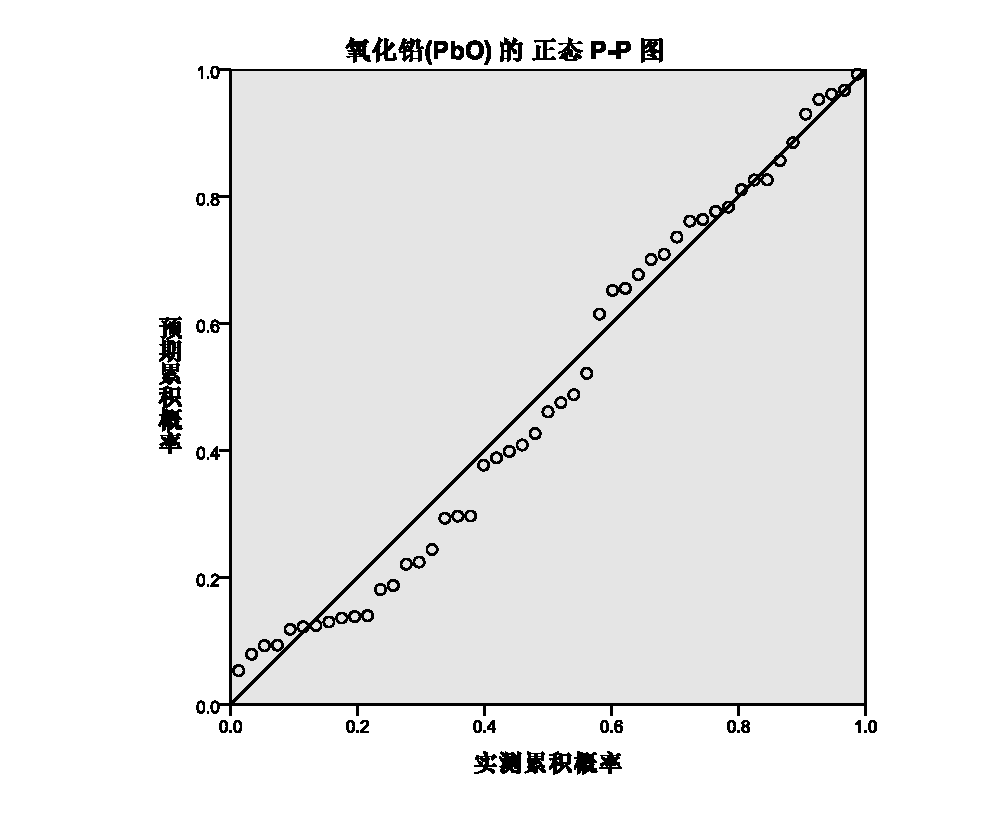
\includegraphics[width=0.49\textwidth]{PbO.eps}
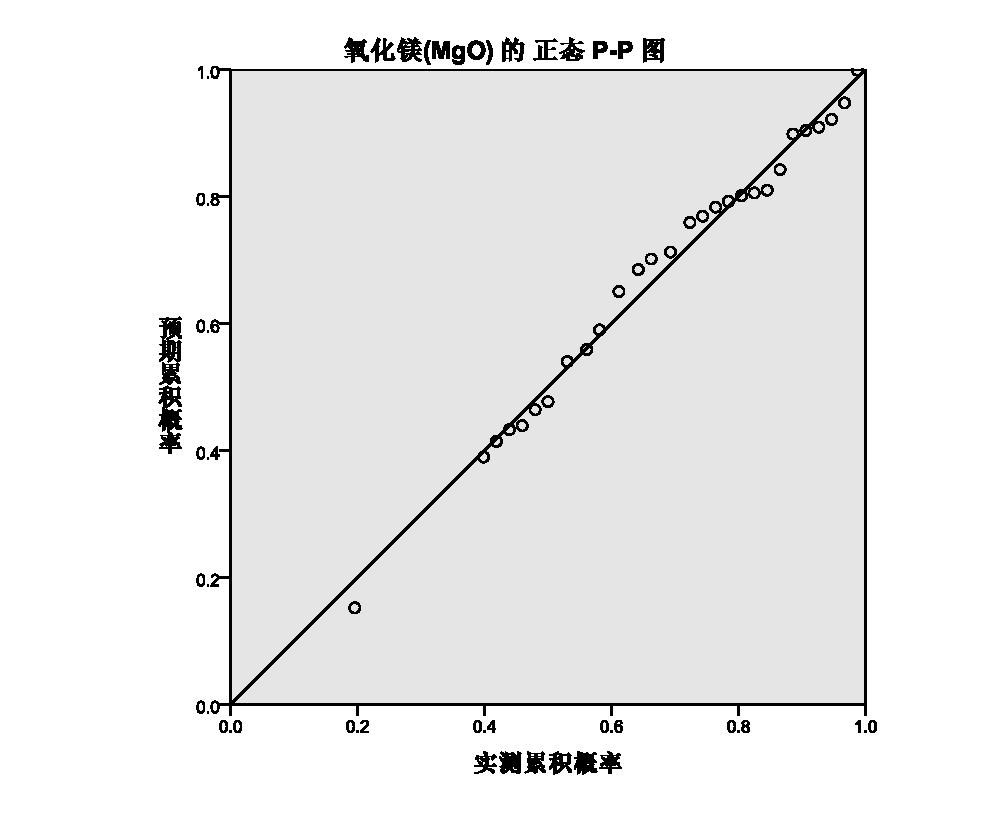
\includegraphics[width=0.49\textwidth]{MgO.eps}
\caption{连续变量正态分布检验结果}
\label{正态分布检验}
\end{figure}

由图可知,数据点分布在对角线附近,说明变量服从正态分布,可以采用二阶段聚类分析模型。

本文使用 SPSS 24.0 进行二阶聚类分析.其中对于分类变量进行代码处理以便调整变量度量.

二阶聚类的结果如表\ref{二阶聚类结果图}所示:\\
\begin{table}[H]
    \centering
    \caption{二阶聚类结果图}
    \label{二阶聚类结果图}
    \begin{tabular}{lllll}
    \hline
   &   &  自动聚类   & ~ & ~ \\ \hline
        聚类数目 & 赤池信息准则 (AIC) & AIC 变化量a & AIC 变化比率b & 距离测量比率c \\ 
        1 & 524.463 & ~ & ~ & ~ \\ 
        2 & 484.317 & -40.146 & 1.000 & 1.492 \\
        3 & 475.872 & -8.445 & 0.210 & 1.566 \\ 
        4 & 490.712 & 14.839 & -0.370 & 1.385 \\ \hline
    \end{tabular}
\end{table}

对二阶聚类分析结果进行分析.该算法依据 AIC 信息准则的判别原则,对客户信息进行聚类
有效性的检测:AIC 越小越好,同时 AIC 变化量距离测量比率值越大,聚类效果越好,以此确定了最优的类别数目.由表 1 可看出聚为 3类效果最佳,它的 AIC 数值较小且距离测量比率较大。\par
二阶聚类的聚物质量图如图\ref{聚物质量图}示:
\begin{figure}[H]
    \centering
    \includegraphics[width=0.49\textwidth]{聚类质量.jpg}
    \caption{二阶聚类的聚物质量图}
    \label{聚物质量图}
\end{figure}

由图可知凝聚和分离的轮廓测量值接近0.8,已达到良好的分离效果,证明二阶聚类分析的合理性。\par
综合上述各图各表,可看出二阶聚类分析将铅钡玻璃分为三类,分别记为亚类4,亚类5,亚类6。\par
\textbf{K-Means++聚类:}基于上述二阶聚类法,已经得出可将铅钡玻璃分为三个亚类,故采用K-Means++聚类分析法,对所有点进行聚类分析,聚类数目设置为3,进而将各个点分别归入三个亚类,亚类划分情况如表\ref{K-Means++聚类划分亚类情况表}所示:
\begin{table}[H]
    \centering
    \caption{K-Means++聚类划分亚类情况表}
    \label{K-Means++聚类划分亚类情况表}
    \begin{tabular}{lllll}
    \hline
        ~ & ~ & 个案数 & 占组合的百分比 & 占总计的百分比 \\ \hline
        聚类 & 1 & 20 & 40.8\% & 40.8\% \\ 
        ~ & 2 & 24 & 49.0\% & 49.0\% \\ 
        ~ & 3 & 5 & 10.2\% & 10.2\% \\ 
        ~ & 组合 & 49 & 100.0\% & 100.0\% \\ \hline
    \end{tabular}
\end{table}

表格显示了系统自动聚类数为3,以及每一类的个案数量及其占比。亚类4共20个样本点,占比40.8\%,亚类5共24个样本点,占比49.0\%,亚类6共5个样本点,占比10.2\%,三个亚类占比均超过10\%,一定程度上反映了亚类划分的合理性。\par
\textbf{合理性证明:}\par
因文物本身仅处于一个亚类,故首先通过对同一玻璃文物的多个采样点所分的亚类进行比对,发现仅03文物的部位1、部位2属于不同亚类,其余文物的各部位点均属于同一亚类。经过数据比对与分析,确定03文物的取样部位2应为无风化文物的表面部分风化点取样。\par
就铅钡亚类分类模型而言,采用R型-Q型综合聚类分析模型进行求解,并通过将结果与原分类结果比照进行检验得到结果,检验结果如表\ref{双模型结果比照表}所示:
\begin{table}[H]
    \centering
    \caption{双模型结果比照表}
    \label{双模型结果比照表}
    \begin{tabular}{lllll}
    \hline
        检验样本数 & 匹配成功数 & 匹配成功率 & 匹配失败数 & 匹配失败率 \\ \hline
        49 & 41 & 83.70\% & 8 & 16.30\% \\ \hline
    \end{tabular}
\end{table}

由表可知此时两种方法的成功匹配率达到83.7\%,仅少量样本亚类划分存在差异,故认为基于二阶聚类分析与K-Means++聚类法的铅钡玻璃亚类划分方法是合理的。\par
就高钾亚类分类模型而言,通过分析算法的数学原理,在找出分类函数后,将样本代入分类函数进行检验,发现均符合分类模型,故认为基于R-Q型聚类分析的高钾玻璃亚类划分方法是合理的。
\subsubsection{铅钡亚类分类灵敏度检验}
在铅钡亚类划分中,我们自行设定了以采样点二氧化硅($SiO_2$)比例、采样点氧化铅($PbO$)比例,采样点氧化钡($BaO$)比例为关键的分类标准,并据此确定了各铅钡玻璃的亚类归属。下面来分析两种算法匹配率对以上三种化学成分变化率的灵敏度。\par
我们使以上三种化学成分在原有数值基础上在其[95\%,105\%]的范围上以1\%的变化率摆动,重新计算两种算法的匹配率,得到结果如图\ref{问题二灵敏度分析}所示。
\begin{figure}[H]
    \centering
    \includegraphics[width=1.0\textwidth]{问题二灵敏度分析.jpg}    \caption{铅钡分类灵敏度分析}
    \label{问题二灵敏度分析}
\end{figure}

由图可知,在关键成分波动范围5\%内,结果匹配率仅波动不超过2\%。当化学成分比原值低时,匹配率随着化学成分的提高而提高,说明此时系统并不稳定,得到的结果是不可靠的。但是当化学成分比原值高时,算法的匹配度保持稳定,故此时系统是稳定的,即所得到的分类结果是正确且稳定的。
\subsection{问题三模型的建立与求解}

\subsubsection{基于逐步判别分析方法的文物类型鉴别模型}

要鉴别表单3中文物的类别,则首先要采用问题2第一小问得到的向量机的分类函数,确认其属于高钾玻璃还是铅钡玻璃。随后使用第二小问的玻璃亚类划分方法,初步确认其所属亚类,并结合综合聚类方法最终判定未知玻璃文物所属类别,其原理图如图\ref{未知判别思路图}所示:
\begin{figure}[H]
    \centering
    \includegraphics[height=6.5cm,width=1.1\textwidth]{对未知玻璃分类思路图.jpg}
    \caption{基于逐步判别分析方法的文物类型鉴别思路图}
    \label{未知判别思路图}
\end{figure}

将表单3的文物数据输入MATLAB,用判别函数

$$\begin{aligned}
c(\tilde{x})=& \sum_{i} \beta_{i} K\left(\boldsymbol{b}_{i}, \tilde{\boldsymbol{x}}\right)+b \\
=& 0.2042 K\left(\boldsymbol{b}_{5}, \tilde{\boldsymbol{x}}\right)+0.7573 K\left(\boldsymbol{b}_{6}, \tilde{\boldsymbol{x}}\right)+0.1703 K\left(\boldsymbol{b}_{21}, \tilde{\boldsymbol{x}}\right)+0.1323 K\left(\boldsymbol{b}_{50}, \tilde{\boldsymbol{x}}\right) \\
&+0.0026 K\left(\boldsymbol{b}_{54}, \tilde{\boldsymbol{x}}\right)+0.7552 K\left(\boldsymbol{b}_{59}, \tilde{\boldsymbol{x}}\right)+0.02417 K\left(\boldsymbol{b}_{60}, \tilde{\boldsymbol{x}}\right)+1.9064
\end{aligned}$$ \\
进行分析,得到A2、A3、A4、A5、A8属于总体$G_1$,即属于铅钡玻璃;A1、A6、A7属于总体$G_2$,即属于高钾玻璃。

\textbf{建立判别函数}

对于高钾玻璃:

\begin{table}[H]
    \centering
    \caption{高钾玻璃分析结果}
    \begin{tabular}{lllll}
    \hline 
        步骤 & a & 容差 & 要除去的 F & 威尔克 Lambda \\ \hline
        1 & 氧化钠($Na_2O$) & 1.000 & 174.840 & ~ \\ 
        2 & 氧化钠($Na_2O$) & 0.988 & 129.293 & 0.123 \\ 
        ~ & 二氧化硅($SiO_2$) & 0.988 & 38.429 & 0.041 \\ 
        3 & 氧化钠($Na_2O$) & 0.859 & 120.346 & 0.070 \\ 
        ~ & 二氧化硅($SiO_2$) & 0.306 & 33.139 & 0.022 \\ 
        ~ & 氧化钾(K2O) & 0.305 & 4.933 & 0.006 \\ \hline
    \end{tabular}
\end{table}

本文采用逐步判别法选择分析变量,经过多次判别分析,最终有3个变量进入判别方程,剔除了11个变量。最终得到高钾玻璃的亚类1,亚类2,亚类3的判别函数分别为:

$$f_{1}(x)=10.527 x_{1}+52.079 x_{2}+13.870 x_{3}-497.073$$

$$f_{2}(x)=8.591 x_{1}+43.493 x_{2}+11.867 x_{3}-334.173 $$

$$f_{3}(x)=10.385 x_{1}+104.139 x_{2}+15.033 x_{3}-567.478$$

对判别函数进行方差检验,得知$P<0.000 5$,说明由筛选出的3个变量组成的判别函数具有显著意义,判别函数对区分高钾玻璃不同亚类差异很显著。作判别时,将样本各化学成分含量代入3个判别函数计算判别函数值,则$f_i=max{f_i}$,即样本属于函数值最大所对应的亚型。

对于铅钡玻璃:

\begin{table}[H]
    \centering
    \caption{铅钡玻璃分析结果}
    \begin{tabular}{llll}
    \hline
        变量 & 容差 & 要除去的 F & 威尔克 Lambda \\ \hline
        二氧化硅($SiO_2$) & 0.863 & 15.669 & 0.077 \\ 
        氧化铜($CuO$) & 0.699 & 35.605 & 0.119 \\ 
        二氧化硫($SO_2$) & 0.588 & 35.052 & 0.118 \\ 
        五氧化二磷($P_2O_5$) & 0.834 & 11.190 & 0.068 \\ 
        氧化钾($K_2O$) & 0.835 & 4.049 & 0.053 \\ \hline
    \end{tabular}
\end{table}
筛选出5个变量进入判别方程,则铅钡玻璃的亚类4,亚类5,亚类6的判别函数分别为: 

$$f_{4}(x)=0.225 x_{1}+3.911 x_{2}+0.811 x_{3}+0.978 x_{4}+0.225 x_{5}-8.291$$

$$f_{5}(x)=0.473 x_{1}-2.338 x_{2}+0.750 x_{3}+0.120 x_{4}+0.930 x_{5}-14.104$$ 

$$f_{6}(x)=0.269 x_{1}-1.556 x_{2}+5.158 x_{3}+0.039 x_{4}+3.662 x_{5}-34.947$$

对判别函数进行方差检验,得知$P<0.000 5$,说明由筛选出的3个变量组成的判别函数具有显著意义,判别函数对区分铅钡玻璃不同亚类差异很显著。作判别时,将样本各化学成分含量代入3个判别函数计算判别函数值,则$f_i=max{f_i}$,即哪个函数值最大就属于哪一种亚型。



将A2、A3、A4、A5、A8的化学成分输入SPSS,使用基于二阶聚类分析与K-Means聚类法的铅钡玻璃亚类划分方法,判断得A2、A3、A4属于亚类4,A5属于亚类5,A8属于亚类6.

将A1、A6、A7的化学成分输入SPSS,采取基于R-Q型聚类分析的高钾玻璃亚类划分方法判断得A6、A7属于亚类1,A1属于亚类2.

其结果与判别方程所得结果一致,证实了文物类别鉴别模型的可信度。

\subsubsection{未知样品分类灵敏度检验}
在对未知样品进行分类的过程中,我们自行筛选出了三个主要变量组成判别函数,并根据判别函数将8个未知玻璃文物归入为5个亚类。下面来分析两个算法匹配率与三个主要变量变化率的灵敏度。\par
我们使以上三种化学成分在原有数值基础上在其[95\%,105\%]的范围上以1\%的变化率摆动,重新计算两种算法的匹配率,得到结果如图\ref{第三问灵敏度分析}所示:
\begin{figure}[H]
    \centering
    \includegraphics[width=1.0\textwidth]{第三问灵敏度分析.jpg}
    \caption{未知样品分类灵敏性检验}
    \label{第三问灵敏度分析}
\end{figure}

由图可知,在关键成分波动范围5\%内,结果匹配率仅波动不超过0.1\%。且当化学成分比原值低时,匹配率随着化学成分的提高而提高,尽管此时匹配率已经很高,也可以认为此时系统并不稳定,认为得到的结果是不可靠的。但是当化学成分比原值高时,算法的匹配度保持稳定,且均超过99.95\%,故此时系统是稳定的,即所得到的分类结果是正确且稳定的。
\newpage
\subsection{问题四模型的建立与求解}
\subsubsection{基于灰色关联分析法的成分关联度分析模型}
因玻璃文物样品化学成分众多,不同种类的玻璃成分差距较大,因此选择灰色关联分析法,以分析玻璃众多化学成分之间的联系关系。采用灰色关联分析法的分析思路如图\ref{灰色关联分析}所示:
\begin{figure}[H]
    \centering
    \includegraphics[width=1\textwidth]{灰色关联分析思路.jpg}
    \caption{采用灰色关联分析法分析化学成分联系的思路}
    \label{灰色关联分析}
\end{figure}
\textbf{确定分析数列}
确定母序列为二氧化硅($SiO_2$)含量,记为$t_0$;子序列为其余有效数据,记为$t_1,t_2,\dots,t_n$,$n\leq 13$。

使用MATLAB对字母序列进行去量钢化,计算子序列中的各个指标对于母序列的关联系数,进而计算出各个指标与母序列的灰色关联度,并计算灰色加权关联度:

   $$ r_{i}=\sum_{k=1}^{n} w_{k} \xi_{i}(k) $$
各个指标变量未给出权重,则各指标变量取相等权重,即$w_{j}=\frac{1}{n}, j=1,2, \cdots, n_{\circ}$

得出结果如表\ref{灰色关联度}所示:

\begin{table}[H]
    \centering
    \begin{tabular}{llllllll}
    \hline
        高钾1 & 高钾2 & 高钾3 &  \multicolumn{2}{c}{铅钡1}  & \multicolumn{2}{c}{铅钡2}   & 铅钡3 \\ \hline
        0.66 & 0.55 & 0.55 & 0.54 & 0.68 & 0.48 & 0.53 & 0.52 \\ 
        0.50 & 0.52 & 0.57 & 0.66 & 0.65 & 0.40 & 0.70 & 0.63 \\ 
        0.51 & 0.54 & 0.54 & 0.59 & 0.73 & 0.37 & 0.73 & 0.55 \\ 
        ~ & 0.47 & 0.44 & 0.60 & 0.41 & 0.40 & 0.77 & 0.60 \\ 
        ~ & 0.54 & ~ & 0.64 & 0.74 & 0.56 & 0.66 & 0.47 \\ 
        ~ & 0.44 & ~ & 0.71 & 0.66 & 0.52 & 0.59 & ~ \\ 
        ~ & 0.37 & ~ & 0.61 & 0.72 & 0.59 & 0.56 & ~ \\ 
        ~ & 0.34 & ~ & 0.75 & 0.71 & 0.64 & 0.57 & ~ \\ 
        ~ & 0.38 & ~ & 0.62 & 0.65 & 0.63 & 0.61 & ~ \\ 
        ~ & 0.41 & ~ & 0.67 & 0.73 & 0.57 & 0.51 & ~ \\ 
        ~ & 0.40 & ~ & ~ & ~ & 0.63 & 0.74 & ~ \\ 
        ~ & ~ & ~ & ~ & ~ & 0.47 & 0.82 \\ \hline
    \end{tabular}
    \caption{灰色加权关联度}
    \label{灰色关联度}
\end{table}

由表可知,铅钡玻璃的亚类内各个成员的相关性相对更强,且不同亚类有着细小差别;高钾玻璃的亚类内各个成员的相关性相对较弱,以亚类2相对明显。\par
就高钾玻璃而言,其亚类内各个成员间相关性相对偏弱。亚类1、亚类3内因成员数目相对偏少,可能导致其内各个成员间相关性相对更高,亚类2内成员数目较多,可能导致其内各个成员间相关性相对更低。\par
就铅钡玻璃而言,其亚类内各个成员间相关性相对偏高,且与高钾玻璃不同,铅钡玻璃的各个亚类内成员间相关性差异微小,不存在亚类突出的情况。
\subsubsection{基于卡方检验的关联关系差异性分析模型}
对于求解关联度分析模型得到的各类文物的加权关联度,按两类为一组进行卡方检验,部分结果如图\ref{卡方检验图}所示:

\begin{figure}[H]
    \centering
    \includegraphics[width=1\textwidth]{第四问卡方检验.png}
    \caption{部分卡方检验图}
    \label{卡方检验图}
\end{figure}

从图\ref{卡方检验图}可以分析出,高钾玻璃的亚类2与铅钡玻璃中的亚类4、5的似然性的渐近显著性为1,可认为差异非常显著;高钾玻璃的亚类3与铅钡玻璃的亚类4、5、6的线性关系渐近显著性均超过0.73,差异较为显著。综上可知,不同玻璃类型间的化学成分关联关系差异较大。

\section{六、模型的评价和推广}
\subsection{模型的评价}
\subsubsection{模型的优点}
\begin{enumerate}
    \item 使用多种聚类分析方法,并让不同方法彼此佐证,使算法稳定性更高,分类更恰当,拟合更准确。
    \item 对多个模型进行灵敏度检验,保证模型在数据一定波动时的可靠性与稳定性。
    \item 模型适用性强,可推广到矿物鉴定、考古挖掘等方面,具有较强的实际价值。
\end{enumerate}
\subsubsection{模型的缺点}
\begin{enumerate}
    \item 问题一预测未风化玻璃的化学成分时未完全考虑所有成分,存在一定的数据残缺
    \item 问题二铅钡玻璃亚类划分的聚类方法在样本数过少时算法适用性较弱。
\end{enumerate}

\subsection{模型的改进}
问题四进行灰色关联分析时,可以针对单样品点,将其所有项变量两两结合计算灰色关联度,随后将每个亚类的各项变量间的灰色关联度取平均值,写出各变量的相关性矩阵,利用多维尺度分析法,结合SPSS软件生成的散点图,使用欧几里得距离公式计算各化学成分之间的关联性。如此可得出各种玻璃亚类的化学成分相关性,便于更准确地比较各类间的化学成分关联关系。

\subsection{模型的推广}
问题二对玻璃文物化学成分的研究过程,本质上是使用多种统计模型对已知样本点的拟合,以及对未知样本点属性的推测。我们可以将模型运用到矿石开采作业中,对新发现的矿石进行成分分析,推测其种类;求解问题三采用的文物类型鉴别模型可以用来鉴别考古发掘中的文物,可推测已风化文物的未风化时成分。
%----------- 参考文献 ----------
\bibliographystyle{unsrt} 
\begin{center}
\bibliography{reference} 
\end{center}

%----------- 附录 ----------
\newpage
\section{附录}

\begin{table}[htbp]
    \centering
    \begin{tabular}{|p{14.0cm}|}

    \hline
    \textbf{附录1} \\ %换行 
    \hline
    .spv 文件是SPSS生成的数据文件 \\ 
     .m文件为MATLAB的代码\\
     .xls文件为本文使用的数据图表\\
     .jpg文件,.png文件, .eps文件为本文插入的图片\\
    \hline
    \end{tabular}
\end{table}
\newpage
\begin{table}[htbp]
    \centering
    \begin{tabular}{|p{14.0cm}|}

    \hline
    \textbf{附录2} \\ 
    \hline
    \lstinputlisting[language=matlab]{K_RCA.m}\\ 
    \lstinputlisting[language=matlab]{K_QCA.m}\\
    \\
    \\
    \hline
    \end{tabular}
\end{table}

\newpage
\begin{table}[htbp]
    \centering
    \begin{tabular}{|p{14.0cm}|}

    \hline
    \textbf{附录2} \\ 
    \hline
    \lstinputlisting[language=matlab]{indiscrimination2.m}\\ 
    \lstinputlisting[language=matlab]{judge.m}
    \\
    \\
    \hline
    \end{tabular}
\end{table}


\end{document}